%%%%%%%%%%%%%%%%%%%%%%%%%%%%%%%%%%%%%%%%%
% Professional Newsletter Template
% LaTeX Template
% Version 1.0 (09/03/14)
%
% Created by:
% Bob Kerstetter (https://www.tug.org/texshowcase/) and extensively modified by:
% Vel (vel@latextemplates.com)
% 
% This template has been downloaded from:
% http://www.LaTeXTemplates.com
%
% License:
% CC BY-NC-SA 3.0 (http://creativecommons.org/licenses/by-nc-sa/3.0/)
%
%%%%%%%%%%%%%%%%%%%%%%%%%%%%%%%%%%%%%%%%%

\documentclass[10pt]{article} % The default font size is 10pt; 11pt and 12pt are alternatives

%%%%%%%%%%%%%%%%%%%%%%%%%%%%%%%%%%%%%%%%%
% Professional Newsletter Template
% Structural Definitions File
% Version 1.0 (09/03/14)
%
% Created by:
% Vel (vel@latextemplates.com)
% 
% This file has been downloaded from:
% http://www.LaTeXTemplates.com
%
% License:
% CC BY-NC-SA 3.0 (http://creativecommons.org/licenses/by-nc-sa/3.0/)
%
%%%%%%%%%%%%%%%%%%%%%%%%%%%%%%%%%%%%%%%%%

%----------------------------------------------------------------------------------------
%	REQUIRED PACKAGES
%----------------------------------------------------------------------------------------

\usepackage{graphicx} % Required for including images
\usepackage{microtype} % Improved typography
\usepackage{multicol} % Used for the two-column layout of the document
\usepackage{booktabs} % Required for nice horizontal rules in tables
\usepackage{wrapfig} % Required for in-line images
\usepackage{float} % Required for forcing figures not to float with the [H] parameter

%------------------------------------------------
% Fonts

\usepackage{charter} % Use the Charter font as the main document font
\usepackage{courier} % Use the Courier font for \texttt (monospaced) only
\usepackage[T1]{fontenc} % Use T1 font encoding

%------------------------------------------------
% List Separation

\usepackage{enumitem} % Required to customize the list environments
\setlist{noitemsep,nolistsep} % Remove spacing before, after and within lists for a compact look

%------------------------------------------------
% Figure and Table Caption Styles

\usepackage{caption} % Required for changing caption styles
\captionsetup[table]{labelfont={bf,sf},labelsep=period,justification=justified} % Specify the table caption style
\captionsetup[figure]{labelfont={sf,bf},labelsep=period,justification=justified, font=small} % Specify the figure caption style
\setlength{\abovecaptionskip}{10pt} % Whitespace above captions

%------------------------------------------------
% Spacing Between Paragraphs

\makeatletter
\usepackage{parskip}
\setlength{\parskip}{6pt}
\newcommand{\@minipagerestore}{\setlength{\parskip}{6pt}}
\makeatother

%----------------------------------------------------------------------------------------
%	PAGE MARGINS AND SPACINGS
%----------------------------------------------------------------------------------------

\textwidth = 7 in % Text width
\textheight = 10 in % Text height
\oddsidemargin = -18pt % Left side margin on odd pages
\evensidemargin = -18pt % Left side margin on even pages
\topmargin = -36pt % Top margin
\headheight = 0pt % Remove the header by setting its space to 0
\headsep = 0pt % Remove the space between the header and top of the page
\parskip = 4pt % Space between paragraph
\parindent = 0.0in % Paragraph indentation
\pagestyle{empty} % Disable page numbering

%----------------------------------------------------------------------------------------
%	COLORS
%----------------------------------------------------------------------------------------

\usepackage[dvipsnames,svgnames]{xcolor} % Required to specify custom colors

\definecolor{altncolor}{rgb}{.8,0,0} % Dark red
%\definecolor{altncolor}{rgb}{.2,.4,.8} % Dark blue
%\definecolor{altncolor}{rgb}{.84,.16,.16} % Red

\usepackage[colorlinks=true, linkcolor=altncolor, anchorcolor=altncolor, citecolor=altncolor, filecolor=altncolor, menucolor=altncolor, urlcolor=altncolor]{hyperref} % Use the color defined above for all links

%----------------------------------------------------------------------------------------
%	BOX STYLES
%----------------------------------------------------------------------------------------

\usepackage[framemethod=TikZ]{mdframed}% Required for creating boxes
\mdfdefinestyle{sidebar}{
    linecolor=black, % Outer line color
    outerlinewidth=0.5pt, % Outer line width
    roundcorner=0pt, % Amount of corner rounding
    innertopmargin=10pt, % Top margin
    innerbottommargin=10pt, % Bottom margin
    innerrightmargin=10pt, % Right margin
    innerleftmargin=10pt, % Left margin
    backgroundcolor=white, % Box background color
    frametitlebackgroundcolor=white, % Title background color
    frametitlerule=false, % Title rule - true or false
    frametitlerulecolor=white, % Title rule color
    frametitlerulewidth=0.5pt, % Title rule width
    frametitlefont=\Large, % Title heading font specification
    font=\small
}

\mdfdefinestyle{intextbox}{
    linecolor=black, % Outer line color
    outerlinewidth=0.5pt, % Outer line width
    roundcorner=10pt, % Amount of corner rounding
    innertopmargin=7pt, % Top margin
    innerbottommargin=7pt, % Bottom margin
    innerrightmargin=7pt, % Right margin
    innerleftmargin=7pt, % Left margin
    backgroundcolor=white, % Box background color
    frametitlebackgroundcolor=white, % Title background color
    frametitlerule=false, % Title rule - true or false
    frametitlerulecolor=white, % Title rule color
    frametitlerulewidth=0.5pt, % Title rule width
    frametitlefont=\Large % Title heading font specification
}

%----------------------------------------------------------------------------------------
%	HEADING STYLE
%----------------------------------------------------------------------------------------

\newcommand{\heading}[2]{ % Define the \heading command
\vspace{#2} % White space above the heading
{\begin{center}\Large\textbf{#1}\end{center}} % The heading style
\vspace{#2} % White space below the heading
}

\newcommand{\BackToContents}{\hyperlink{contents}{{\small Back to Contents}}} % Define a command for linking back to the contents of the newsletter % Include the document which specifies all packages and structural customizations for this template
\usepackage{soul}
\setuldepth{Berlin}
\usepackage{lettrine}
\usepackage{amsmath}
\usepackage{nicefrac}
\usepackage{booktabs}
\usepackage{graphicx}
\usepackage{subfig}
\usepackage[usestackEOL]{stackengine}
%\usepackage{libertine}
\usepackage{fancyhdr}
% Turn on the style
\pagestyle{fancy}
% Clear the header and footer
\fancyhead{}
\fancyfoot{}
\renewcommand{\headrulewidth}{0pt}
% Set the right side of the footer to be the page number
\fancyfoot[r]{\thepage}
%\usepackage{showframe}


\setlength{\footskip}{1\baselineskip}

\begin{document}
	
	%----------------------------------------------------------------------------------------
	%	HEADER IMAGE
	%----------------------------------------------------------------------------------------
	
	%\begin{figure}[H]
	%\centering
\includegraphics[width=0.3\linewidth]{logo.png}
	%\end{figure}
	\centering \textsc{Poseidon: Open source Syringe Pump and Microscope}
	%----------------------------------------------------------------------------------------
	%	SIDEBAR - FIRST PAGE
	%----------------------------------------------------------------------------------------
	
	\begin{minipage}[t]{.30\linewidth} % Mini page taking up 30% of the actual page
		\begin{mdframed}[style=sidebar,frametitle={}] % Sidebar box
			
			%----------------------------------------------------------
			
			%\centerline {\rule{.75\linewidth}{.25pt}} % Horizontal line
			
			%-----------------------------------------------------------
			\textbf{\large Poseidon Quick Facts: }
			\centerline {\rule{.75\linewidth}{.25pt}} % Horizontal line			
			
			\begingroup
			\setstackgap{S}{2pt}
			\setlength{\tabcolsep}{3pt} % Default value: 6pt
			\renewcommand{\arraystretch}{1.5} % Default value: 1
			\begin{tabular}{@{}rl@{}}
				\textbf{\emph{Operation:}} & infuse \& withdraw \\
				\textbf{\emph{Total Cost:}} &$<$\$400\\
				\textbf{\emph{Print time:}} & 23hr\\
				\textbf{\emph{Build time: }} & 30min\\
				\textbf{\emph{Syringe:}} & BD Plastic 1-60mL\\
				\textbf{\emph{Dist Units:}} & mm, mL, $\mu$L\\
				\textbf{\emph{Time units:}} & sec, min, hr\\
				\textbf{\emph{Pos. Tol:}} & $\pm$ 2\%\\
				\textbf{\emph{Pos. Range:}} & 0-150mm\\
				\textbf{\emph{Speed Range:}} & 60 $\mu$m-60 mm/min\\
				\textbf{\emph{Max Rate:}} & 33.24 mL/min\\
				\textbf{\emph{Min Rate:}} & 1.03 $\mu$L/min\\
				\textbf{\emph{Microscope:}} & excellent\\
			\end{tabular}
		\endgroup
			
			
			%\centerline {\rule{.75\linewidth}{.25pt}} % Horizontal line
			\vspace{6px}
			\textbf{\large Experiments are easy:} 
			\centerline {\rule{.75\linewidth}{.25pt}} % Horizontal line			
			
			Assuming components are connected and powered:
			
			\begin{enumerate}[leftmargin=*]
				\raggedright
				\item Launch the GUI by typing \texttt{python gui.pu}
				\item Load \texttt{testing.txt} by pressing \texttt{File -> Load Settings}
				\item Select the arduino port 
				\item Send the settings to the controller by pressing \texttt{send to controller}
				\item In the run tab, enable the pumps you want to run, and enter their displacements
				\item Press \texttt{run} on the run tab to start your experiment
				\item Pause or stop at any time by pressing \texttt{pause} or \texttt{stop}
			\end{enumerate}
			
			%-----------------------------------------------------------
			\vspace{10px}
			\textbf{\large Get started:}
			
			\centerline {\rule{.75\linewidth}{.25pt}} % Horizontal line			
			Check out the project page which has all of the files as well as detailed instructions on how to build (and hack) the system!
			\url{https://pachterlab.github.io/poseidon/}
			
			%-----------------------------------------------------------
			
%			\captionof*{table}{Table Caption}
%			\begin{tabular}{llr}
%				\toprule
%				\multicolumn{2}{c}{Name} \\
%				\cmidrule(r){1-2}
%				First & Last & Grade \\
%				\midrule
%				John & Doe & $7.5$ \\
%				Richard & Miles & $2$ \\
%				\bottomrule
%			\end{tabular}
			
			%-----------------------------------------------------------
			
		\end{mdframed}
	\end{minipage}\hfill % End the sidebar mini page 
	%
	%----------------------------------------------------------------------------------------
	%	MAIN BODY - FIRST PAGE
	%----------------------------------------------------------------------------------------
	%
	\begin{minipage}[t]{.66\linewidth} % Mini page taking up 66% of the actual page
		
		\hypertarget{firstnews}{\heading{An overview of the Poseidon System}{6pt}} % \hypertarget provides a label to reference using \hyperlink{label}{link text}
		\lettrine[lraise=0.1, nindent=0em, slope=-.5em]{T}{he} Poseidon pumps and microscope are a customizable open source alternative to commercial systems that costs less than \$400 and can be assembled in under an hour. It uses 3D printed parts and common components that can be easily purchased from Amazon or other retailers. The microscope and pumps can be used together in microfluidics experiments, but the pumps can also be connected to a computer and used independently for other experiments.
		

		
%		\begin{center}
%			\parbox[t]{.70\linewidth}{\emph{Principles of Open Hardware Design include: Modular, Hackable, Standalone/PC Interface, Minimize Dependencies, Simple \& Robust, Easy to Build, Affordable, Benchmarked}}
%		\end{center}
		
		\begin{wrapfigure}[9]{r}[0pt]{0pt} % In-line figure with text wrapping around it
			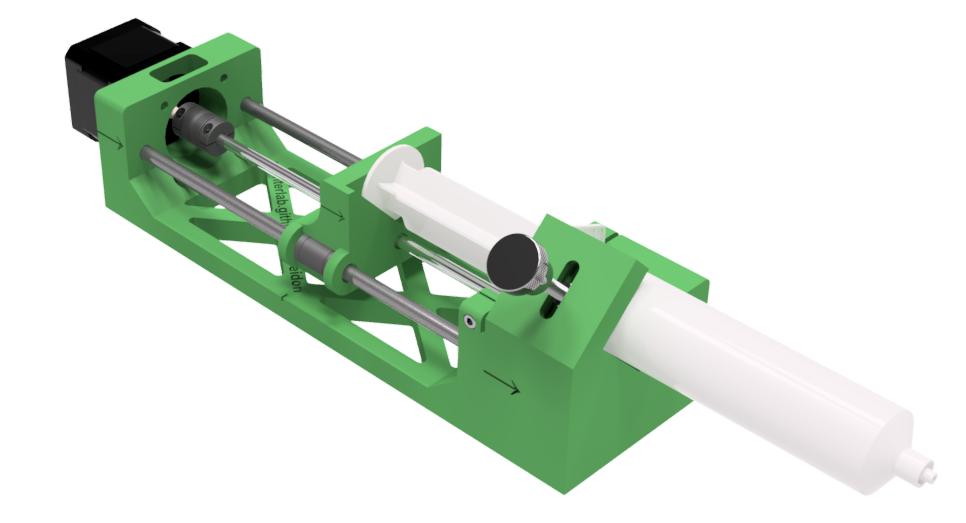
\includegraphics[width=0.4\textwidth]{img/pump-ortho.png}
		\end{wrapfigure}
		The pumps are driven by an Arduino with a CNC shield and up to three pumps can be run at once. Each pump has a stepper motor that drives a lead screw which in turn moves a sled that is mounted on linear bearings. The displacement of the sled moves the syringe forward or backward allowing the user to dispel or intake liquid.


		\begin{wrapfigure}[9]{l}[0pt]{0pt} % In-line figure with text wrapping around it
			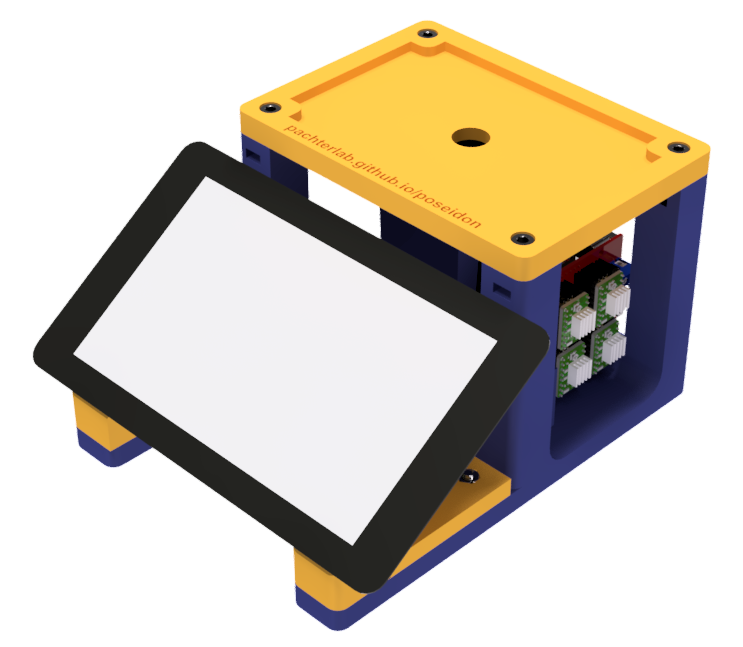
\includegraphics[width=0.33\textwidth]{img/cam-ortho.png}
		\end{wrapfigure}
		
The controller station uses a Raspberry Pi with a touchscreen to connect to the Arduino and microscope via USB. Because the microscope and Arduino use USB connections, the they can alternatively be connected to any computer instead.  
		

	
		
		%-----------------------------------------------------------
		
		\hypertarget{secondnews}{\heading{On the development of the Poseidon System}{6pt}} % \hypertarget provides a label to reference using \hyperlink{label}{link text}
		
		The Poseidon system was designed to be customizable. It uses the Raspberry Pi and Arduino electronics boards, which are supported by a strong ecosystem of open source hardware and software, facilitating the implementation of new functionalities. The following components developed for the Poseidon system are made available:
		\begin{enumerate}
			\item Computer Aided Design (CAD) files of the 3D printed components
			\item Pump controller software and Graphical User Interface (GUI) to control the Arduino
			 \item Arduino firmware used to drive the motors
		\end{enumerate}

		
		The 3D printed components can be fabricated on any desktop fused filament fabrication (FFF) 3D printer. They were designed using Autodesk Fusion 360, a proprietary CAD software that offers free academic licenses. To modify the 3D models the user can either use Fusion 360 or any other CAD software.
		
		The GUI was created using Qt designer, a drag and drop application for organizing buttons that allows the used to easily make modifications. This GUI is used to interface with a Python script that controls both the microscope and Arduino via USB. 
		
		The pumps are driven by an Arduino board that interprets commands sent via USB and sends the proper signal to control the stepper motor movement. The user can take advantage of this by developing custom movement patterns using built-in Arduino functions.
		
	\end{minipage} % End the main body - first page mini page
	
	%----------------------------------------------------------------------------------------
	%	MAIN BODY - SECOND PAGE
	%----------------------------------------------------------------------------------------
	
	\begin{minipage}[t]{.66\linewidth} % Mini page taking up 66% of the actual page
		
		\hypertarget{thirdnews}{\heading{On the licensing of the Poseidon System}{6pt}} % \hypertarget provides a label to reference using \hyperlink{label}{link text}
		
		\begin{multicols}{2} % Two-column layout
			This is still TBD.
		\end{multicols}
		
		\centerline {\rule{.75\linewidth}{.25pt}} % Horizontal line	
		\hypertarget{quotation}{{\textbf{\large User Quotes}}} % \hypertarget provides a label to reference using \hyperlink{label}{link text}
		
		\begin{quote}
			\raggedright \textsl{Finally a reliable, inexpensive, and hackable system that I can use for my Drop Seq experiments.} \\ \raggedleft--- \textrm{J. Gehring (Post Doc)}
		\end{quote}
		
		\begin{quote}
			\raggedright \textsl{I loved how easy the system was to setup!} \\ \raggedleft--- \textrm{L. Pachter (P.I.)}
		\end{quote}
	
		\begin{quote}
			\raggedright \textsl{The system comes really close to beating out the Harvard Pumps, I can't wait to work on these pumps and contribute to the open source community.} \\ \raggedleft--- \textrm{E. D. V. Beltrame (Graduate Student)}
		\end{quote}
	

		
		%----------------------------------------------------------------------------------------
		
	\end{minipage}\hfill % End of the main body - second page mini page
	\begin{minipage}[t]{.30\linewidth} % Mini page taking up 30% of the actual page
		
		%----------------------------------------------------------------------------------------
		%	SIDEBAR - SECOND PAGE
		%----------------------------------------------------------------------------------------
		
		\begin{mdframed}[style=sidebar,frametitle={}] % Sidebar box
			
			\heading{Tech Specs}{0pt}
			
			\centerline {\rule{.75\linewidth}{.25pt}} % Horizontal line	
			\begingroup
			\setstackgap{S}{3pt}
			\setlength{\tabcolsep}{3pt} % Default value: 6pt
			\renewcommand{\arraystretch}{1.5} % Default value: 1
			\begin{tabular}{@{}rl@{}}
				\textbf{\emph{Motor Type: }} & Nema 17\\
				\textbf{\emph{Motor Steps: }} & 200/rev\\
				\textbf{\emph{Screw pitch: }} & 0.8 mm/rev\\
				\textbf{\emph{Microstep: }} & $\nicefrac{1}{2} \,\, \nicefrac{1}{8}\,\, \nicefrac{1}{16}\,\, \nicefrac{1}{32}$\\
				\textbf{\emph{Dist per step: }} & 4 $\mu$m\\
				\textbf{\emph{Arduino Power: }} & 12V DC @ 2A\\
				\textbf{\emph{Raspi Power: }} & 5V DC @ 1A\\
			\end{tabular}
			\endgroup
			
		\end{mdframed}\hfill
		
		%----------------------------------------------------------------------------------------
		

		\begin{minipage}[t]{.95\linewidth}
			\raggedright\textbf{Contact Us:}\\
			Sina Booeshaghi\\
			Pachter Lab, California Institute of Technology Pasadena, CA.\\
			\href{email}{abooeshab@caltech.edu}\\
			\href{labpage}{pachterlab.github.io/poseidon}
		\end{minipage}
		
		%----------------------------------------------------------------------------------------
		
	\end{minipage} % End of the sidebar mini page
	
	%----------------------------------------------------------------------------------------
	\begin{minipage}[t]{1\linewidth} % Mini page taking up 66% of the actual page
	
	\hypertarget{thirdnews}{\heading{Appendix A: Images of the Poseidon system}{6pt}} % \hypertarget provides a label to reference using \hyperlink{label}{link text}
			\centerline {\rule{.75\linewidth}{.25pt}} % Horizontal line			
\end{minipage}\hfill % End of the main body - second page mini page
\begin{center}
\begin{figure}[h]
	\centering
	\begin{tabular}{cc}
		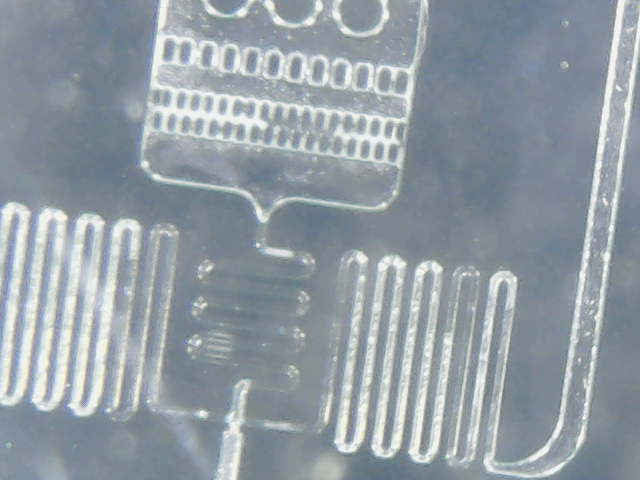
\includegraphics[width=.25\linewidth]{img/blue.png} &   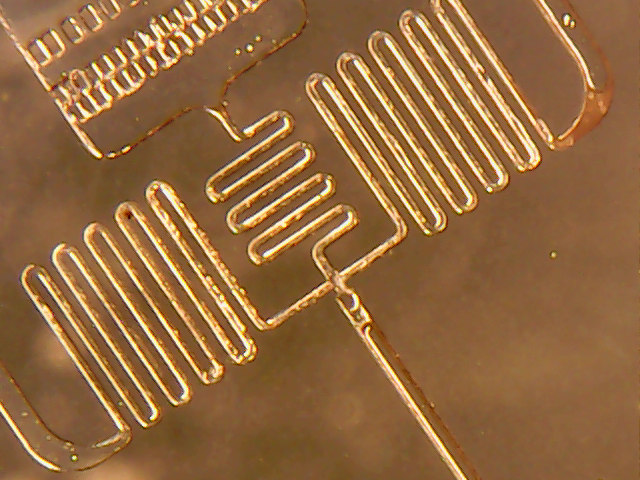
\includegraphics[width=.25\linewidth]{img/yellow.png} \\
		(a) USB Microscope w/ LED & (b) USB Microscope w/o LED \\[6pt]
		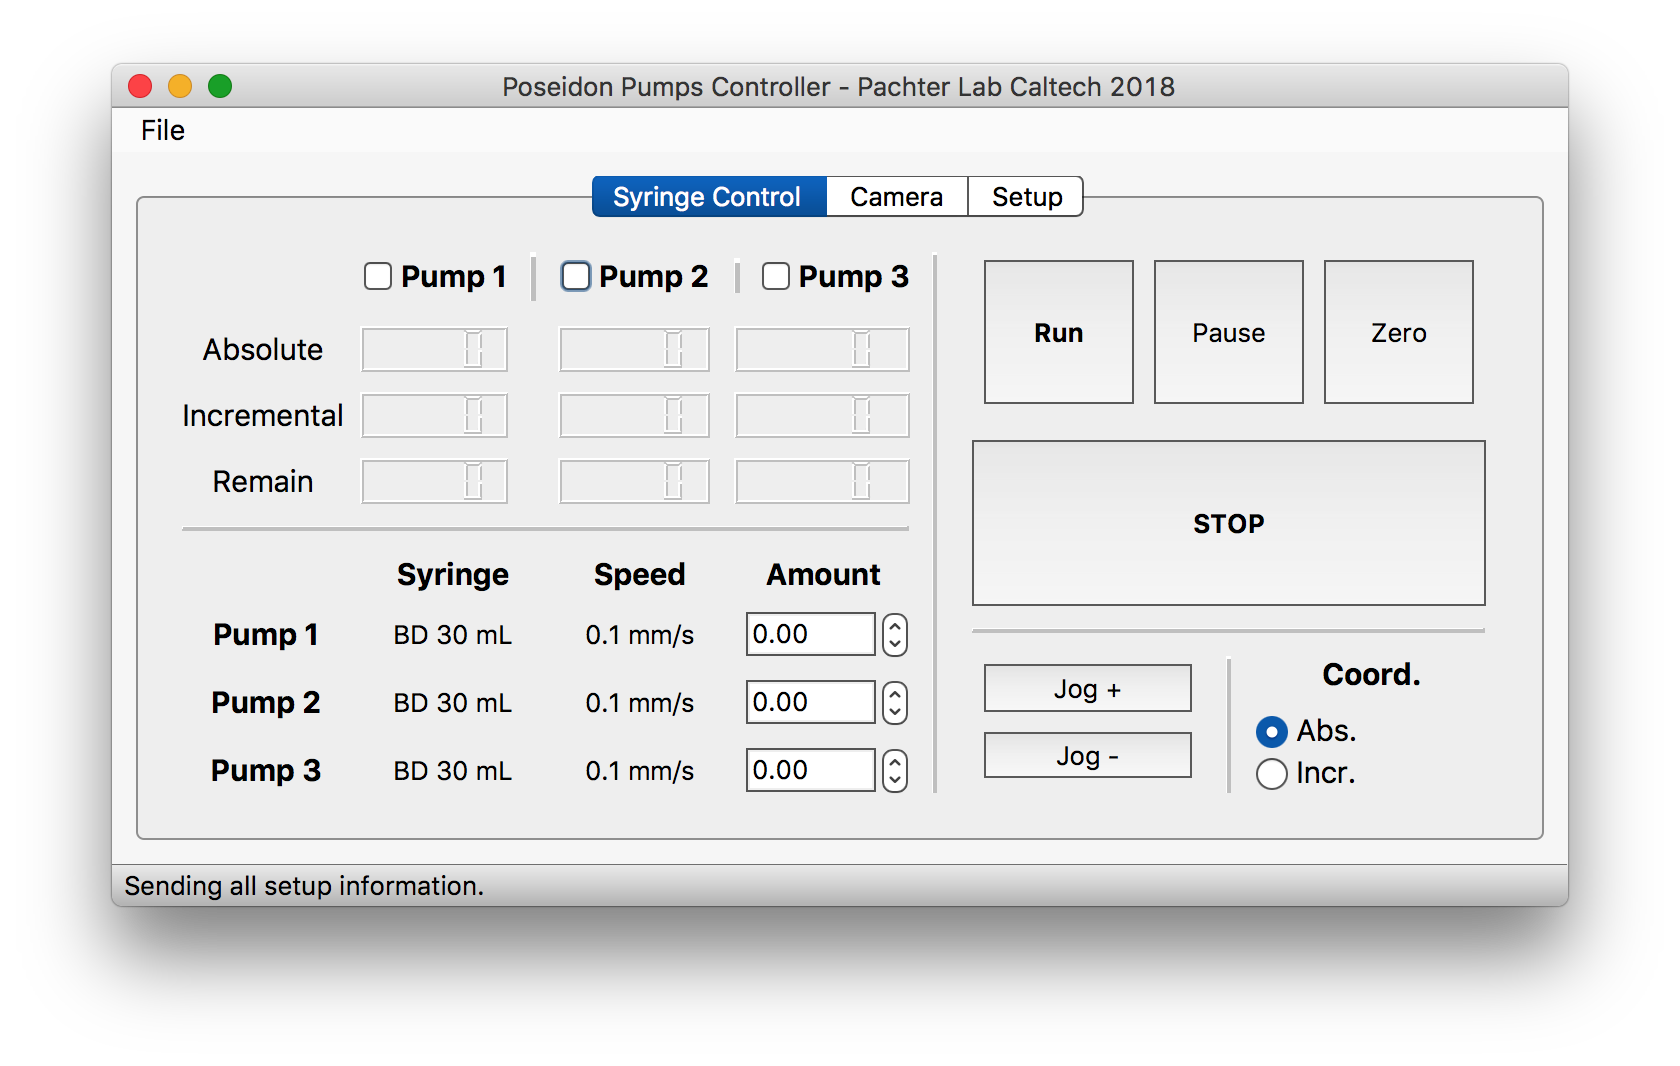
\includegraphics[width=.35\linewidth]{img/run.png} &   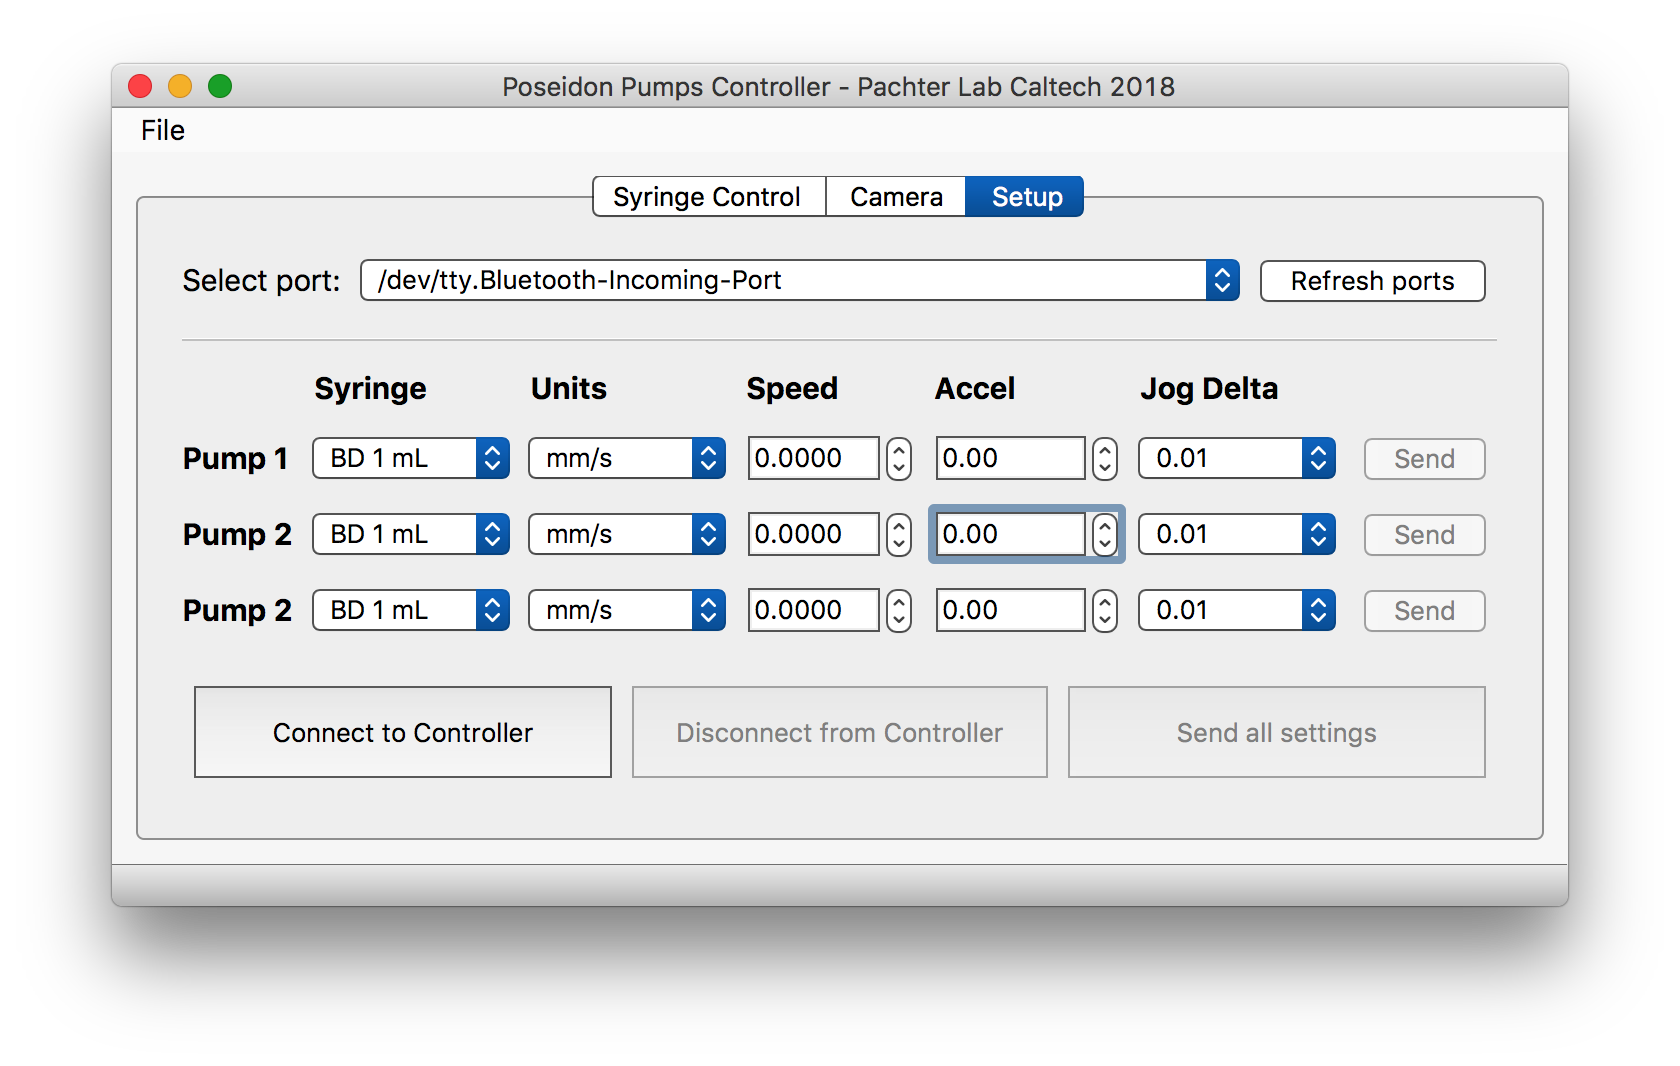
\includegraphics[width=.35\linewidth]{img/settings.png} \\
		(c) GUI run page & (d) GUI settings page \\[6pt]
		\multicolumn{2}{c}{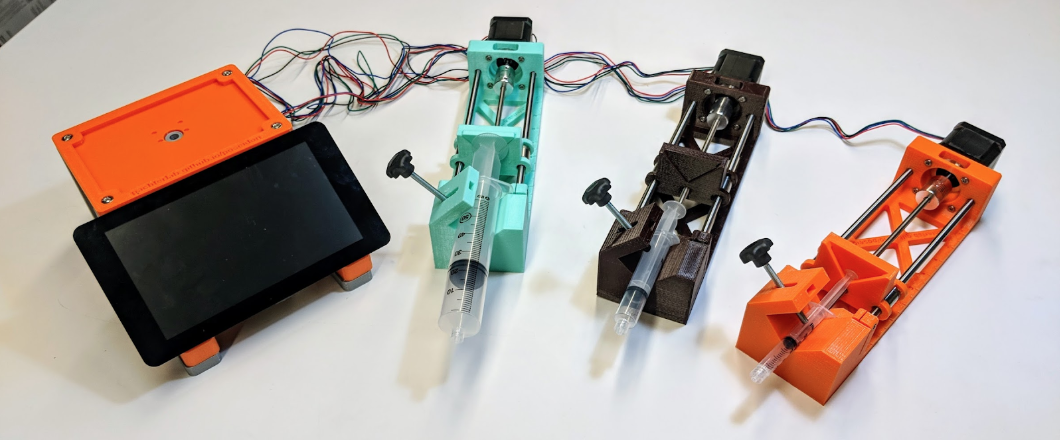
\includegraphics[width=.5\linewidth]{img/all.png} }\\
		\multicolumn{2}{c}{(e) The whole system}
	\end{tabular}
\end{figure}
\end{center}
\end{document} 